\documentclass[12pt]{article}
\usepackage[a4paper,top=2cm,bottom=2.2cm,left=3cm,right=3cm,marginparwidth=1.75cm]{geometry}
\usepackage{amsmath,amsthm,amssymb}
\usepackage[spanish]{babel}
\usepackage{listings}
\usepackage{csvsimple,booktabs}
\usepackage{filecontents}
\usepackage{amsmath}
\usepackage{graphicx} % figuras
\usepackage{subfigure} % subfiguras
\usepackage{color}
\usepackage{cite}
\definecolor{mygreen}{rgb}{0,0.6,0}
\definecolor{mygray}{rgb}{0.5,0.5,0.5}
\definecolor{mymauve}{rgb}{0.58,0,0.82}
\usepackage[colorinlistoftodos]{todonotes}
\usepackage[colorlinks=true, allcolors=blue]{hyperref}
\usepackage{movie15}
\usepackage[utf8]{inputenc}
\lstdefinestyle{tt}{language=Python, literate= {á}{{\'a}}1 {ó}{{\'o}}1 {ñ}{{\~n}}1, breaklines=true, basicstyle={\small}, commentstyle=\color{red}, frame=single, extendedchars=true, otherkeywords={True, False}, keywordstyle=\color{mymauve}, columns=flexible, stringstyle=\color{mygreen}, breakatwhitespace=true, numbers=left, numberstyle=\scriptsize\color{mygray}, tabsize=3, rulecolor=\color{black}}
\lstdefinestyle{rm}{language=R, commentstyle=\color{mygray}, keywordstyle=\color{blue}, stringstyle=\color{mygreen}, breakatwhitespace=true, breaklines=true, columns=flexible, extendedchars=true, literate={ó}{{\'o}}1 {ú}{{\'u}}1 {ñ}{{\~n}}1 }
\begin{document}
\title{{\LARGE \textbf{Experimentos con el algoritmo de Floyd-Warshall en \texttt{python}}}\\ {\large Yessica Reyna Fernández}\\{\large Flujo en Redes}}
\maketitle
\section{Introducción}
En base a la estructura ya usada por los grafos en la práctica anterior[1], se 
\section{Grafo circular base}
Primeramente con respecto a la posición de los nodos, se posicionan en forma de circunferencia, entonces se realiza la transformación a coordenadas en radianes para la circunferencia a formar; a continuación se debe definir en ese caso la posición del angulo en donde ira cada punto para esta transformación por lo cual se deberá tomar una medida equitativa para la cantidad de nodos que se tiene, tomando en cuenta la ecuación paramétrica de la circunferencia con centro en $(a,b)$ donde $x=a+rCos(t)$ y $y=b+rSen(t)$ con $t\in[0,2\pi]$, definiendo lo siguiente como parte básica del grafo:
\begin{lstlisting}[style=tt]
angulo=2*pi/n #n=cantidad de nodos
r=0.3 #radio fijo de la circunferencia
c=(0.5,0.5) #posición del centro de la circunferencia
self.pos[v] = (c[0]+(r * cos(angulo * v)), c[1]+(r* sin(angulo * v))) #dentro de la función nodoscrear() con v=indice del nodo a crear
\end{lstlisting}
Ahora bien hablando de la forma de trazar las aristas entre nodos se mide en forma de un parámetro $k$, el cual varia dependiendo de la cantidad de nodos; por lo que se busca que cada vez que se corra el código las repeticiones que habrá de cada tamaño este dada por el valor $ \lfloor n/2 \rfloor $ ademas de que el valor de $k$ realiza las conexiones entre nodos; asimismo se define \texttt{E[(u,v)]} como las distancias euclidianas entre cada par de nodos y \texttt{vecinos[v].add(i+(j+1))} lo que agrega al nodo $i+(j+1)$  entre los vecinos de $v$, todo esto descrito en lo siguiente:
\begin{lstlisting}[style=tt]
def conecta(self, k) #función de conexiones en aristas
	for j in range(k): #recorrer tamaño de k
		for i in range(len(self.V)): #recorriendo cada nodo
			if i< (len(self.V)-(j+1)): #siempre que el indice no pase el valor k
				self.E[(i, i+(j+1))] = self.E[(i+(j+1), i)]=self.euclidiana(i,(i+(j+1)))
				self.vecinos[i].add(i+(j+1))
				self.vecinos[i+(j+1)].add(i)
\end{lstlisting}
En relación con esto se define la función para integrar aristas aleatorias al grafo que depende de una probabilidad que aumenta con el valor de $k$, agregando esa nueva arista siempre que no se encuentre considerada en el, ademas de que su probabilidad para entrar al grafo sea mas pequeña que un numero que se genera aleatoriamente:
\begin{lstlisting}[style=tt]
prob=2**-(k)
def conectaaleatorio(self, prob)
	if m is not w and (m,w) not in self.E:
		if random()< prob:
			self.E[(m,w)]=self.E[(w,m)]=self.euclidiana(m,w)
			self.vecinos[m].add(w)
			self.vecinos[w].add(m)
\end{lstlisting}
Así pues esto definiría lo mas básico por elaborar par aun grafo base circular, tratando en las siguientes secciones otros aspectos que se pueden agregar al grafo.
\section{Promedios de distancias}
Como se ha tratado en practicas anteriores, el algoritmo de Floyd-Warshall[2] crea un vector con todos los pares de distancias entre un par de puntos dados $u$ y $v$.\\
Por lo cual se puede considerar como característica en el grafo lo que seria el promedio de distancias entre nodos, tomando la suma de distancias de todos los pares de nodos dados obteniendo así este parámetro que varia dependiendo de la cantidad de nodos, esto es, $D= \frac{\sum_{i=1}^n d[i]}{n}$, donde \texttt{d[i]} es el vector de las distancias tomado del algoritmo de Floyd-Warshall.\\ Donde todo lo ya dicho se desglosa en las siguiente lineas de código:
\begin{lstlisting}[style=tt]
def promediodistancias(self):
	self.suma = 0
	for key, value in self.d.items():
		self.suma= self.suma+value
	return self.suma/n
\end{lstlisting}
Acto seguido a esto se define una nueva función matemática, la cual en relación a los valores de $n$ y de $k$, se crea una cota superior al valor de la distancia promedio que se calculo con anterioridad.\\
Hablando un poco mas de ella, esta se calcula en base a la longitud del vector de distancias, el cual crece conforme al valor de $n$, entre el cociente de la mitad de las interacciones que hay de nodos y la longitud de la circunferencia.\\Dicho de otra manera, se mostrara a continuación las lineas de código pertenecientes a la descripción de la formulación de la cota superior para la normalizacion de las distancia promedio del grafo conforme a la cantidad de nodos y el valor de interacción entre ellos $k$, asimismo nos indica si para algun valor de $n$ y de $k$ no se llega a cumplir el valor de la cota y se pueda realizar el ajuste de esta:
\begin{lstlisting}[style=tt]
def cota(self):
	circumferencelength= 2*(pi)*r
	supremo=(((n**2)-n)/((0.5)*k))*circumferencelength
	if supremo> self.suma/n:
		return (self.suma/n)/supremo
	else:
		print(n, k)
		print("No es buena cota")
\end{lstlisting}
\section{Densidad de cluster}
Como otro rasgo a denotar para un grafo se puede considerar la densidad de cada uno de sus cluster o grupo su equivalente en español, el cual indica el numero de conexiones que debería existir por grupo que forma cada uno de los nodos individualmente, es decir, quienes de sus vecinos esta conectado entre ellos mismos.\\
Formulando esto matemáticamente se obtendría un coeficiente de densidad de grupo en un rango de $(0,1)$ con la siguiente formula: $C=\frac{2m}{n(n-1)!}$.\\ Obteniendo esto en el código con las siguiente lineas, en donde al formar una doble iteración en la lista de los vecinos de $v$ se evita poner el dos de la formula y dividiendo al final entre la cantidad de nodos generados:
\begin{lstlisting}[style=tt]
def promclusters(self):
	csuma=0
	for v in range(len(self.V)):
		m=0
		for i in self.vecinos[v]:
			for b in self.vecinos[v]:
				if b in self.vecinos[v]:
					m += 1
					csuma += m/(n*(n-1))
	return csuma/len(self.V)
\end{lstlisting}\pagebreak
\section{Resultados}
El objetivo principal de la practica era verificar el comportamiento del tiempo que se toma el algoritmo implementado en resolverse y comprobar así que se sigue manteniendo el mismo comportamiento de tiempo computacional empleado por el algoritmo de Floyd-Warshall, asimismo como interpretar los datos obtenidos por las nuevas características del grafo agregadas para uso de esta practica y así demostrar algún tipo de comportamiento que se relacione entre la cantidad de nodos a considerar y las variaciones de conexiones entre pares de nodos.\\
Entre las siguientes figuras se mostrara la relación de los tiempos tomados para los diferentes cantidades de nodos que se vera en la figura \ref{Figura 1:}, como también se verán los gráficos generados para las distancias promedio en la figura \ref{Figura 2:} y la figura  y las densidades de cluster realizados para cada cantidad de nodos.
\begin{figure}[h!]
	\centering
	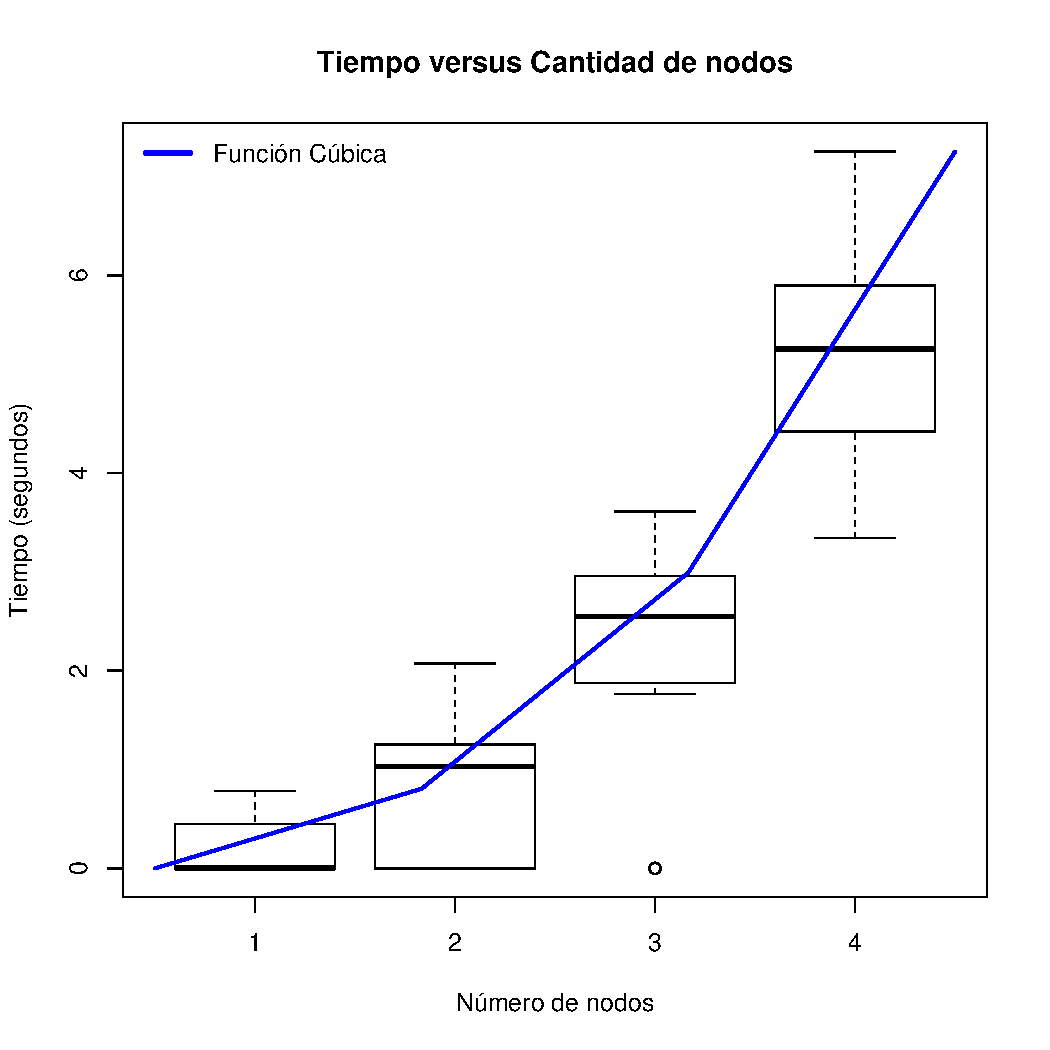
\includegraphics[width=0.6\textwidth]{TiempovsN}
	\caption{Tiempo versus Cantidad de nodos\label{Figura 1:}}
\end{figure}
\begin{figure}[h!]
	\centering
	\subfigure[$n=60$.]{\includegraphics[width=0.70\textwidth]{imgen60}}
	\subfigure[$n=90$.]{\includegraphics[width=0.70\textwidth]{imgen90}}
	\caption{Distancia promedio/cota y densidad de cluster.}\label{Figura 2:}
\end{figure}
\begin{figure}[h!]
	\centering
	\subfigure[$n=60$.]{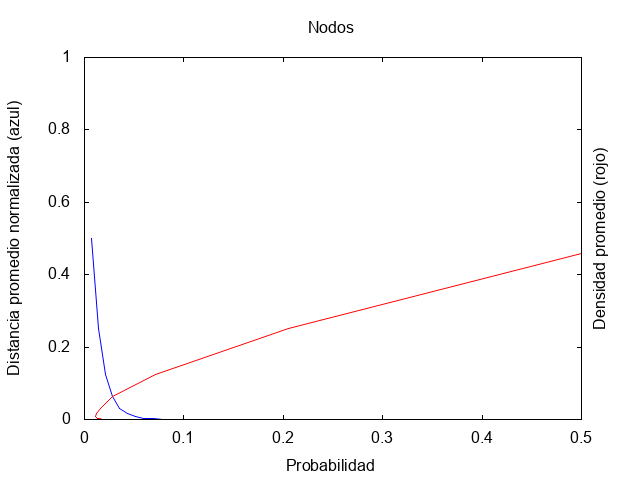
\includegraphics[width=0.70\textwidth]{imgen}}
	\subfigure[$n=90$.]{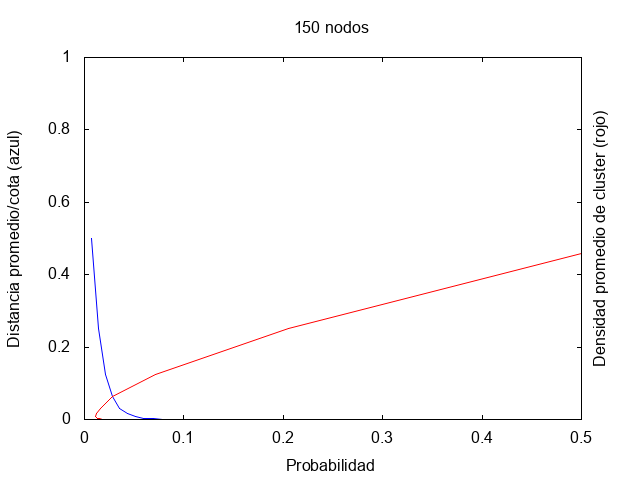
\includegraphics[width=0.70\textwidth]{imagen150}}
	\caption{Distancia promedio/cota y densidad de cluster.}\label{Figura 2:}
\end{figure}
\end{document}